\documentclass[11pt, a4papper]{report}
\usepackage{amsthm}
\usepackage{amssymb, amsmath}
\usepackage{array}
\usepackage[romanian]{babel}
\usepackage{bm}
\usepackage{enumerate}
\usepackage{float}
\usepackage{geometry}
\usepackage{graphicx}
\usepackage{listings}
\usepackage{longtable}
\usepackage[utf8]{inputenc}
\usepackage{listings}
\usepackage{colortbl}
\usepackage[svgnames]{xcolor}
\usepackage{bbding}
\usepackage{pifont}
\usepackage{wasysym}
\usepackage{subcaption}
\DeclareMathOperator*{\minimize}{argmin}
\DeclareMathOperator*{\limi}{lim}
\usepackage[linesnumbered,ruled,vlined]{algorithm2e}
\usepackage{algpseudocode}

\newcommand\mycommfont[1]{\footnotesize\ttfamily\textcolor{blue}{#1}}
\SetCommentSty{mycommfont}

\SetKwInput{KwInput}{Input}                
\SetKwInput{KwOutput}{Output}              

\theoremstyle{plain}
\newtheorem{theorem}{Theorem}

\theoremstyle{definition}
\newtheorem{definition}{Definition}

\theoremstyle{definition}
\newtheorem{lemma}{Lemma}

\newcolumntype{M}[1]{>{\centering\arraybackslash}m{#1}}

\lstset{language=R,
    basicstyle=\small\ttfamily,
    stringstyle=\color{DarkGreen},
    otherkeywords={0,1,2,3,4,5,6,7,8,9},
    morekeywords={TRUE,FALSE},
    deletekeywords={data,frame,length,as,character},
    keywordstyle=\color{blue},
    commentstyle=\color{DarkGreen},
}


\theoremstyle{proposition}
\newtheorem{proposition}{Proposition}

 \geometry{
 a4paper,
 total={160mm,257mm},
 left=30mm,
 right=20mm,
 top=20mm,
 bottom=20mm,
 }
 
\setcounter{tocdepth}{4}
\setcounter{secnumdepth}{4}
\renewcommand{\baselinestretch}{1.25}
 
\graphicspath{ {Images/} }

 

\addto\captionsromanian{
  \renewcommand{\contentsname}%
    {Contents}%
}

\addto\captionsportuguese{\renewcommand{\refname}{References}}

\begin{document}
\begin{center}

\vspace*{.06\textheight}
{\scshape\large {``Alexandru Ioan Cuza" University of Iaşi}\par}\vspace{0.3cm} 
\textsc{\large {Master of computational optimization}}\\[0.3cm] 
\textbf{\textsc{\large {FACULTY OF COMPUTER SCIENCE }}}\\[1.3cm] 


\vspace{0.4cm}
\textsc{\large {Advanced Software Engineering Techniques 2019 Project}}\\[0.1cm]
\textsc{\large { - State of the art - }}\\[2.7cm]

\vspace{0.6cm}
{\LARGE \bfseries {Freesound Audio Tagging 2019}\par}
\vspace{0.2cm} 
{\Large \bfseries {Automatically recognize sounds and apply tags of varying natures}\par}


\vspace{4.4cm}

\begin{center}
\textsc{\large Proposed by: Cojocaru Gabriel-Codrin}\\
\textsc{\large Dinu Sergiu Andrei} \\
\textsc{\large Luncașu Bogdan Cristian} \\
\textsc{\large Racoviță Mădălina-Alina} \\
\textsc{\large Vîntur Cristian} \\
[3.1cm]
\textsc{\large Scientific coordinators}: {\textsc{\large PhD Associate Professor Adrian Iftene}} \\
{\textsc{\large PhD Associate Professor Mihaela Elena Breaban}}
\end{center}
\end{center}
\newpage

%----------------------------------------------------------------------------------------
%	Table of contents
%----------------------------------------------------------------------------------------

\addcontentsline{toc}{chapter}{Contents}

\tableofcontents

\newpage

%----------------------------------------------------------------------------------------
%	Introduction
%----------------------------------------------------------------------------------------


\addcontentsline{toc}{chapter}{I. Introduction}
\chapter*{I. Introduction}
\

%----------------------------------------------------------------------------------------
%	Competition's description
%----------------------------------------------------------------------------------------
\addcontentsline{toc}{section}{I.1. Competition's description}
\section*{I.1. Competition's description}
\

One year ago, \textbf{Freesound} and \textbf{Google’s Machine Perception} hosted an audio tagging competition challenging Kagglers to build a general-purpose auto tagging system. This year they’re back and taking the challenge to the next level with multi-label audio tagging, doubled number of audio categories, and a noisier than ever training set. \cite{1}

\begin{center}
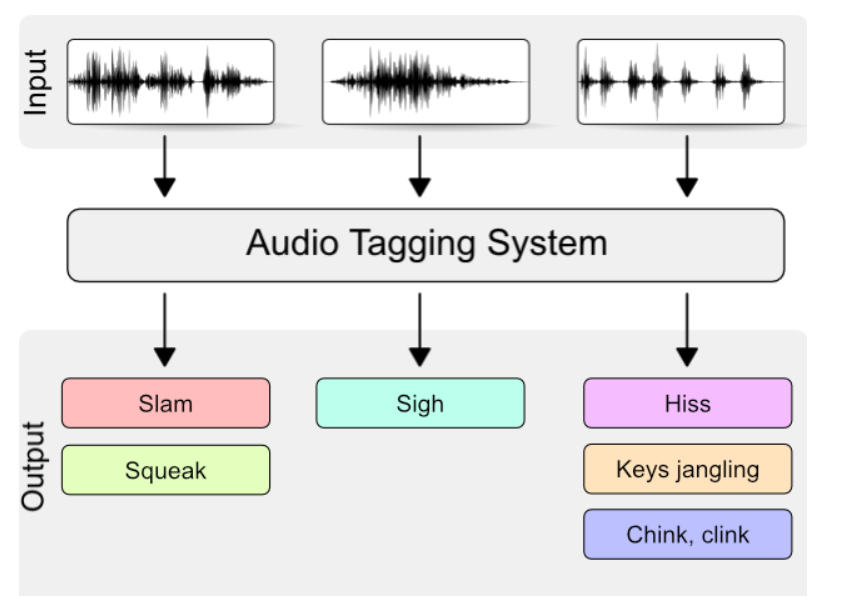
\includegraphics[width=16.5cm,height=9cm,keepaspectratio]{competiton-description.png}
\end{center}

Here's the background: \textbf{Some sounds are distinct and instantly recognizable, like a baby’s laugh or the strum of a guitar}. Other sounds are difficult to pinpoint. If you close your eyes, could you tell the difference between the sound of a chainsaw and the sound of a blender?
\\

Because of \textbf{the vastness of sounds we experience}, \textit{no reliable automatic general-purpose audio tagging systems exist}. A significant amount of manual effort goes into tasks like annotating sound collections and providing captions for non-speech events in audiovisual content.
\\

To tackle this problem, Freesound (an initiative by MTG-UPF that maintains a collaborative database with over 400,000 Creative Commons Licensed sounds) and Google Research’s Machine Perception Team (creators of AudioSet, a large-scale dataset of manually annotated audio events with over 500 classes) have teamed up to develop the dataset for this new competition.
\\

\textbf{To win} this competition, Kagglers will develop an \textbf{algorithm to tag audio data automatically} using a diverse vocabulary of 80 categories.
\\

If successful, these systems could be used for several applications, ranging from \textbf{automatic labelling of sound collections} to \textbf{the development of systems that automatically tag video content} or recognize sound events happening in real time.

%----------------------------------------------------------------------------------------
%	Motivation
%----------------------------------------------------------------------------------------
\addcontentsline{toc}{section}{I.2. Motivation}
\section*{I.2. Motivation}
\

Current machine learning techniques require large and varied datasets in order to provide good performance and generalization. However, manually labelling a dataset is time-consuming, which limits its size. Websites like Freesound or Flickr host large volumes of user-contributed audio and metadata, and labels can be inferred automatically from the metadata and/or making predictions with pre-trained models. Nevertheless, these automatically inferred labels might include a substantial level of label noise.
\\

The main research question addressed in this competition is \textbf{how to adequately exploit a small amount of reliable, manually-labeled data, and a larger quantity of noisy web audio data in a multi-label audio tagging task with a large vocabulary setting}. In addition, since the data comes from different sources, the task encourages domain adaptation approaches to deal with a potential domain mismatch.

%----------------------------------------------------------------------------------------
%	Timeline
%----------------------------------------------------------------------------------------
\addcontentsline{toc}{section}{I.3. Timeline}
\section*{I.3. Timeline}
\

\begin{itemize}
\item \textbf{June 3, 2019 11:59 PM UTC} - Entry deadline. You must accept the competition rules before this date in order to compete.
\item \textbf{June 3, 2019 11:59 PM UTC} - Team Merger deadline. This is the last day participants may join or merge teams.
\item \textbf{June 11, 2019 11:59 AM UTC} - Final submission deadline.
\end{itemize}

%----------------------------------------------------------------------------------------
%	Dataset description
%----------------------------------------------------------------------------------------


\addcontentsline{toc}{chapter}{II. Dataset description}
\chapter*{II. Dataset description}
\

%----------------------------------------------------------------------------------------
%	Audio Dataset
%----------------------------------------------------------------------------------------
\addcontentsline{toc}{section}{II.1. Audio Dataset}
\section*{II.1. Audio Dataset}
\

The dataset used in this challenge is called \textbf{FSDKaggle2019}, and it employs audio clips from the following sources:
\begin{itemize}
\item Freesound Dataset (\textbf{FSD}): a dataset being collected at the \textbf{MTG-UPF} based on \textbf{Freesound} content organized with the AudioSet Ontology
\item  The soundtracks of a pool of Flickr videos taken from the \textbf{Yahoo Flickr Creative Commons 100M dataset (YFCC)}
\end{itemize}


The audio data is labeled using a vocabulary of 80 labels from \textbf{Google’s AudioSet Ontology} \cite{2}, covering diverse topics: Guitar and other Musical instruments, Percussion, Water, Digestive, Respiratory sounds, Human voice, Human locomotion, Hands, Human group actions, Insect, Domestic animals, Glass, Liquid, Motor vehicle (road), Mechanisms, Doors, and a variety of Domestic sounds. 


%----------------------------------------------------------------------------------------
%	Ground Truth Labels
%----------------------------------------------------------------------------------------
\addcontentsline{toc}{section}{II.2. Ground Truth Labels}
\section*{II.2. Ground Truth Labels}
\

The ground truth labels are provided at the clip-level, and express the presence of a sound category in the audio clip, hence can be considered weak labels or tags. Audio clips have variable lengths (roughly from 0.3 to 30s, see more details below).
\\

The audio content from \textbf{FSD} has been \textbf{manually labeled} by humans following a data labeling process using the \textbf{Freesound Annotator platform}. Most labels have inter-annotator agreement but not all of them. More details about the data labeling process and the Freesound Annotator can be found in \cite{3}.
\\

The \textbf{YFCC soundtracks} were labeled using automated heuristics applied to the audio content and metadata of the original Flickr clips. Hence, a substantial amount of label noise can be expected. The label noise can vary widely in amount and type depending on the category, including in- and out-of-vocabulary noises. More information about some of the types of label noise that can be encountered is available in \cite{4}.


%----------------------------------------------------------------------------------------
%	Format and License
%----------------------------------------------------------------------------------------
\addcontentsline{toc}{section}{II.3. Format and License}
\section*{II.3. Format and License}
\

All clips are provided as uncompressed PCM 16 bit, 44.1 kHz, mono audio files. All clips used in this competition are released under Creative Commons (CC) licenses, some of them requiring attribution to their original authors and some forbidding further commercial reuse. In order to be able to comply with the CC licenses terms, a full list of audio clips with their associated licenses and a reference to the original content (in Freesound or Flickr) will be published at the end of the competition. Until then, the provided audio files can only be used for the sole purpose of participating in the competition.
\\

%----------------------------------------------------------------------------------------
%	Train set
%----------------------------------------------------------------------------------------
\addcontentsline{toc}{section}{II.4. Train set}
\section*{II.4. Train set}
\

The train set is meant to be for system development. The idea is to limit the supervision provided (i.e., the manually-labeled data), thus promoting approaches to deal with label noise. The train set is composed of two subsets as follows:

%----------------------------------------------------------------------------------------
%	Curated subset
%----------------------------------------------------------------------------------------
\addcontentsline{toc}{subsection}{II.4.1. Curated subset}
\subsection*{II.4.1. Curated subset}
\

The curated subset is a small set of manually-labeled data from FSD.
\begin{itemize}
\item \textbf{Number of clips/class}: 75 except in a few cases (where there are less)
\item \textbf{Total number of clips}: 4970
\item \textbf{Avge number of labels/clip}: 1.2
\item \textbf{Total duration}: 10.5 hours
\end{itemize}
\

The duration of the audio clips ranges from 0.3 to 30s due to the diversity of the sound categories and the preferences of Freesound users when recording/uploading sounds. It can happen that a few of these audio clips present additional acoustic material beyond the provided ground truth label(s).


%----------------------------------------------------------------------------------------
%	Noisy subset
%----------------------------------------------------------------------------------------
\addcontentsline{toc}{subsection}{II.4.2. Noisy subset}
\subsection*{II.4.2. Noisy subset}
\

The noisy subset is a larger set of noisy web audio data from Flickr videos taken from the \textbf{YFCC dataset} \cite{6}.
\begin{itemize}
\item \textbf{Number of clips/class}: 300
\item \textbf{Total number of clips}: 19815
\item \textbf{Avge number of labels/clip}: 1.2
\item \textbf{Total duration}: ~80 hours
\end{itemize}
\

The duration of the audio clips ranges from 1s to 15s, with the vast majority lasting 15s.
\\

Considering the numbers above, per-class data distribution available for training is, for most of the classes, 300 clips from the noisy subset and 75 clips from the curated subset, which means 80% noisy - 20% curated at the clip level (not at the audio duration level, considering the variable-length clips).

%----------------------------------------------------------------------------------------
%	Test set
%----------------------------------------------------------------------------------------
\addcontentsline{toc}{section}{II.5. Test set}
\section*{II.5. Test set}
\

The test set is used for system evaluation and consists of manually-labeled data from FSD. Since most of the train data come from YFCC, some acoustic domain mismatch between the train and test set can be expected. All the acoustic material present in the test set is labeled, except human error, considering the vocabulary of 80 classes used in the competition.
\\

The test set is split into two subsets, for the public and private leaderboards. In this competition, the submission is to be made through Kaggle Kernels. Only the test subset corresponding to the public leaderboard is provided (without ground truth).

%----------------------------------------------------------------------------------------
%	Files
%----------------------------------------------------------------------------------------
\addcontentsline{toc}{section}{II.6. Files}
\section*{II.6. Files}
\

\begin{center}
\begin{footnotesize}
\begin{tabular}{ | M{4.6cm} | m{10cm} | } 
\hline
\rowcolor[rgb]{0.8588, 0.2823, 0.1725}\multicolumn{2}{|c|}{\textcolor{white}{The structure of the data}} \\
\hline
\cellcolor[rgb]{0.6745, 0.686, 0.709}
\textit{\textbf{\textcolor{white}{train\_curated.csv }}}& \cellcolor[rgb]{0.965, 0.969, 0.967}  {ground truth labels for the curated subset of the training audio files (see Data Fields below)} \\
\hline
\cellcolor[rgb]{0.6745, 0.686, 0.709}
\textit{\textbf{\textcolor{white}{train\_noisy.csv}}} & \cellcolor[rgb]{0.965, 0.969, 0.967}  { ground truth labels for the noisy subset of the training audio files (see Data Fields below)} \\
\hline
\cellcolor[rgb]{0.6745, 0.686, 0.709}
\textit{\textbf{\textcolor{white}{sample\_submission.csv}}}& \cellcolor[rgb]{0.965, 0.969, 0.967}  { a sample submission file in the correct format, including the correct sorting of the sound categories; it contains the list of audio files found in the test.zip folder (corresponding to the public leaderboard)} \\
\hline
\cellcolor[rgb]{0.6745, 0.686, 0.709}
\textit{\textbf{\textcolor{white}{train\_curated.zip }}} & \cellcolor[rgb]{0.965, 0.969, 0.967}  { a folder containing the audio (.wav) training files of the curated subset}\\
\hline
\cellcolor[rgb]{0.6745, 0.686, 0.709}
\textit{\textbf{\textcolor{white}{train\_noisy.zip }}} & \cellcolor[rgb]{0.965, 0.969, 0.967}  { a folder containing the audio (.wav) training files of the noisy subset}\\
\hline
\cellcolor[rgb]{0.6745, 0.686, 0.709}
\textit{\textbf{\textcolor{white}{test.zip}}} & \cellcolor[rgb]{0.965, 0.969, 0.967}  {a folder containing the audio (.wav) test files for the public leaderboard}\\
\hline
\end{tabular}
\end{footnotesize}
\end{center}


%----------------------------------------------------------------------------------------
%	Columns
%----------------------------------------------------------------------------------------
\addcontentsline{toc}{section}{II.7. Columns}
\section*{II.7. Columns}
\
Each row of the train\_curated.csv and train\_noisy.csv files contains the following information:
\begin{itemize}
\item \textbf{fname}: the audio file name, eg, 0006ae4e.wav
\item \textbf{labels}: the audio classification label(s) (ground truth). Note that the number of labels per clip can be one, eg, Bark or more, eg, "Walk\_and\_footsteps,Slam".
\end{itemize}

%----------------------------------------------------------------------------------------
%	Dataset problems
%----------------------------------------------------------------------------------------
\addcontentsline{toc}{section}{II.8. Dataset problems}
\section*{II.8. Dataset problems}

Detected corrupted files in the curated train set
The following 5 audio files in the curated train set have a wrong label, due to a bug in the file renaming process: \textbf{f76181c4.wav}, \textbf{77b925c2.wav}, \textbf{6a1f682a.wav}, \textbf{c7db12aa.wav}, \textbf{7752cc8a.wav}
\\

The audio file \textbf{1d44b0bd.wav} in the curated train set was found to be corrupted (contains no signal) due to an error in format conversion.

%----------------------------------------------------------------------------------------
%	Sound classification predictive models
%----------------------------------------------------------------------------------------


\addcontentsline{toc}{chapter}{IV. Sound classification predictive models}
\chapter*{IV. Sound classification predictive models}
\

%----------------------------------------------------------------------------------------
%	Models brief description
%----------------------------------------------------------------------------------------
\addcontentsline{toc}{section}{IV.1. Models brief description}
\section*{IV.1. Models brief description from different Kaggle approaches}
\

\textbf{Kaggle} \cite{9} is an online community of data scientists and machine learners. Since Kaggle allows users to find and publish data sets, explore and build models in a web-based data-science environment, work with other data scientists and machine learning engineers, and enter competitions to solve data science challenges, it \textbf{can be used also as a source of inspiration when solving different tasks machine learning related}. We extracted some of the predictive models that we have found in the public kernels that were attached to the subject competition.

%----------------------------------------------------------------------------------------
%	Bidirectional LSTM for audio labeling with Keras
%----------------------------------------------------------------------------------------
\addcontentsline{toc}{subsection}{IV.1.1. Bidirectional LSTM for audio labeling with Keras}
\subsection*{IV.1.1. Bidirectional LSTM for audio labeling with Keras}
\

\textbf{Long short-term memory (LSTM)} is an artificial \textbf{recurrent neural network (RNN)} architecture used in the field of deep learning. Unlike standard feedforward neural networks, LSTM has feedback connections. It can not only process single data points (such as images), but also entire sequences of data (such as speech or video). For example, LSTM is applicable to tasks such as \textbf{unsegmented, connected handwriting recognition or speech recognition}. \textbf{LSTM}in its core, \textit{preserves information from inputs that has already passed through it using the hidden state}.
\\

\textbf{Unidirectional LSTM} only \textbf{preserves information of the past} because the only inputs it has seen are from the past. Using \textbf{bidirectional} will \textbf{run your inputs in two ways, one from past to future and one from future to past} and what differs this approach from unidirectional is that \textbf{in the LSTM that runs backwards you preserve information from the future} and using the two hidden states combined you are able in any point in time to preserve information from both past and future.
\\

What they are suited for is a very complicated question but BiLSTMs show very good results as they can understand context better, but this can be explain through a simple example. Lets say we try to predict the next word in a sentence, on a high level what a unidirectional LSTM will see is:
\vspace{0.5cm}
\begin{lstlisting}[language=Python]
The boys went to ....
\end{lstlisting}
\vspace{0.5cm}

And will try to predict the next word only by this context, with bidirectional LSTM you will be able to see information further down the road for example

\vspace{0.5cm}

\begin{lstlisting}[language=Python]
# Forward LSTM:

The boys went to ...

# Backward LSTM:

... and then they got out of the pool
\end{lstlisting}
\vspace{0.5cm}

You can see that using the information from the future it could be easier for the network to understand what the next word is. 

\begin{center}
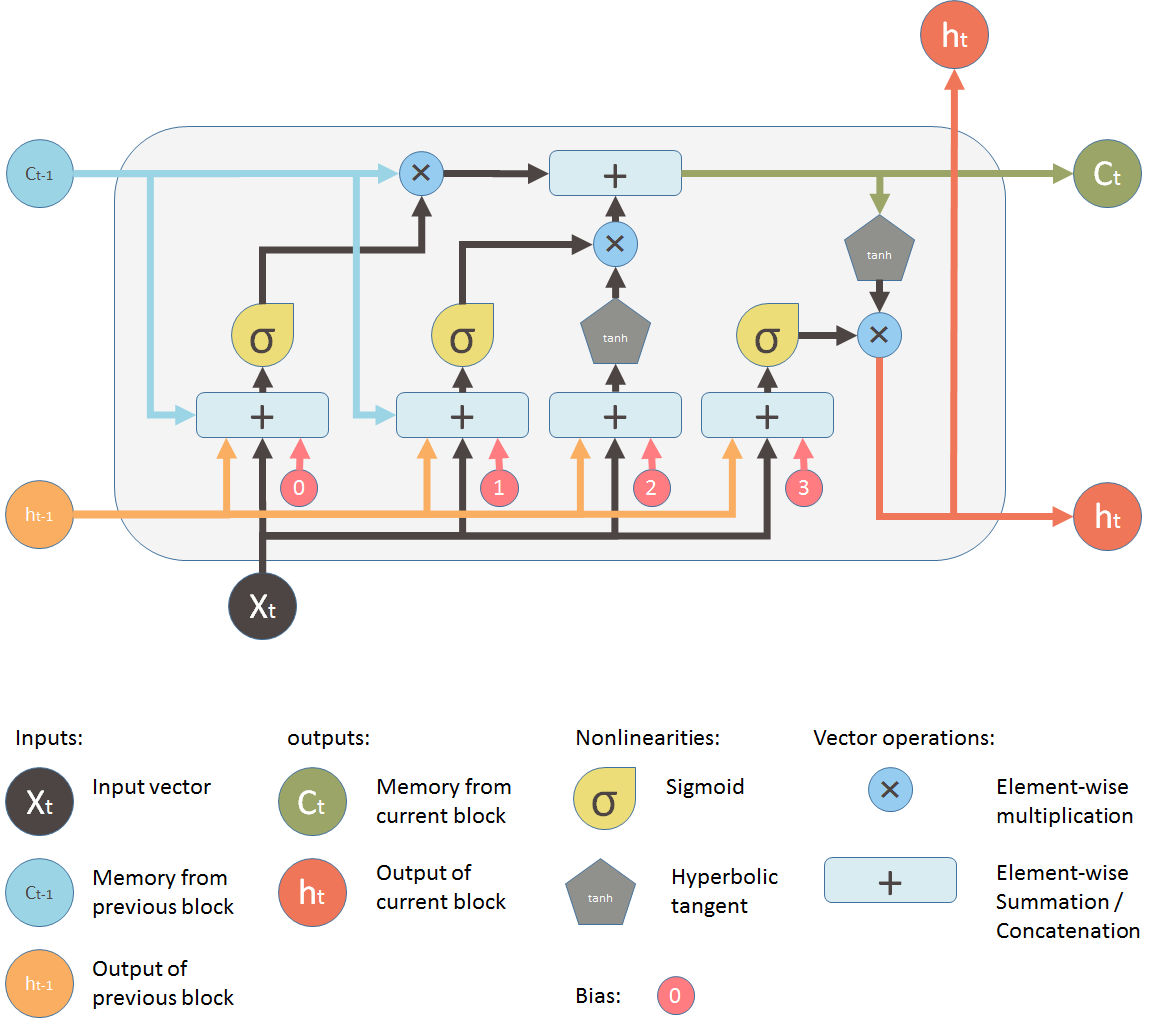
\includegraphics[width=16cm,height=13cm,keepaspectratio]{LSTM.png}
\end{center}
\begin{center}
\textbf{Fig. IV.1.1.a}: \textit{Overview LSTM}
\end{center}

In a public Kaggle kernel  \cite{8} it was used the following architecture for the \textbf{Freesound classification problem} inspired from an article named \textit{Convolutional RNN: an Enhanced Model for
Extracting Features from Sequential Data} \cite{11}.
%\vspace{0.5cm}

\begin{lstlisting}[language=Python]
# Neural network model
input_shape = (636,128)
optimizer = Adam(0.005, beta_1=0.1, beta_2=0.001, amsgrad=True)
n_classes = 80

model = Sequential()
model.add(Bidirectional(CuDNNLSTM(256, return_sequences=True),
	  input_shape=input_shape))
model.add(Attention(636))
model.add(Dropout(0.2))
model.add(Dense(400))
model.add(ELU())
model.add(Dropout(0.2)) 
model.add(Dense(n_classes, activation='softmax'))
model.compile(loss='categorical_crossentropy',
              optimizer=optimizer,
              metrics=['acc'])
\end{lstlisting}
\
% \vspace{0.5cm}

Another likely model that develops a biird sound classification problem and uses bidirectional
LSTM neural networks had the following architecture:
\begin{center}
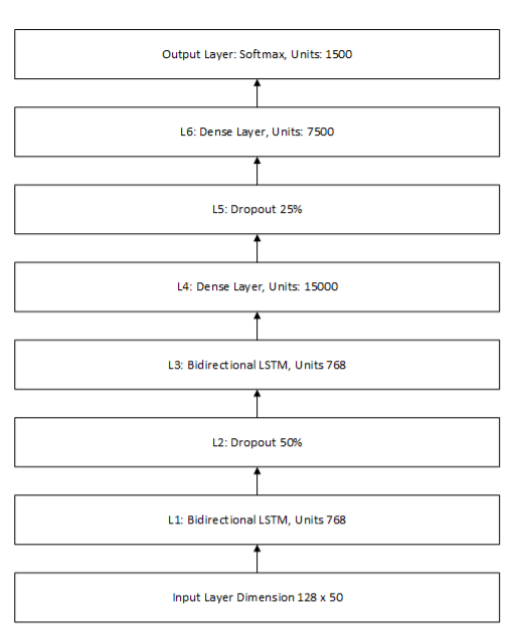
\includegraphics[width=16cm,height=11cm,keepaspectratio]{architecture-bidirect-LSTM.png}
\end{center}
\begin{center}
\textbf{Fig. IV.1.1}: \textit{Architecture bidirectional LSTM. \cite{10}}
\end{center}

%----------------------------------------------------------------------------------------
%	Evaluation metric
%----------------------------------------------------------------------------------------
\addcontentsline{toc}{section}{IV.2. Evaluation metric}
\section*{IV.2. Evaluation metric}
\

The task consists of \textbf{predicting the audio labels (tags) for every test clip}. Some test clips bear one label while others bear several labels. The predictions are to be done at the clip level, i.e., no start/end timestamps for the sound events are required.
\\

The primary competition metric will be \textbf{label-weighted label-ranking average precision} \cite{7}(lwlrap, pronounced "Lol wrap"). This \textbf{measures the average precision of retrieving a ranked list of relevant labels} for each test clip (i.e., the system ranks all the available labels, then the precisions of the ranked lists down to each true label are averaged). This is a generalization of the mean reciprocal rank measure for the case where there can be multiple true labels per test item. The novel "label-weighted" part means that the overall score is the average over all the labels in the test set, where each label receives equal weight (by contrast, plain lrap gives each test item equal weight, thereby discounting the contribution of individual labels when they appear on the same item as multiple other labels).
\\

The formula for label-ranking average precision (LRAP) is as follows:
\begin{equation}
LRAP(y, \widehat{f}) = \frac{1}{n_{samples}}\sum\limits_{i=0}^{n_{samples}-1}\frac{1}{\left\lVert y_i\right\rVert_0} \sum\limits_{j:y_{ij}=1} \frac{|\mathcal{L}_{ij}|}{rank_{ij}}
\end{equation}

\begin{lstlisting}[language=Python]
def calculate_overall_lwlrap_sklearn(truth, scores):
    """Calculate the overall lwlrap using sklearn.metrics.lrap."""
    # sklearn doesn't correctly apply weighting to samples with no labels
    # so just skip them.
    sample_weight = np.sum(truth > 0, axis=1)
    nonzero_weight_sample_indices = np.flatnonzero(sample_weight > 0)
    overall_lwlrap = label_ranking_average_precision_score(
        truth[nonzero_weight_sample_indices, :] > 0, 
        scores[nonzero_weight_sample_indices, :], 
        sample_weight=sample_weight[nonzero_weight_sample_indices])
    return overall_lwlrap
\end{lstlisting}

%----------------------------------------------------------------------------------------
%	Application prototype
%----------------------------------------------------------------------------------------


\addcontentsline{toc}{chapter}{V. Application prototype}
\chapter*{V. Application prototype}
\

%----------------------------------------------------------------------------------------
%	Use cases
%----------------------------------------------------------------------------------------
\addcontentsline{toc}{section}{V.1. Use cases}
\section*{V.1. Use cases}
\
\begin{itemize}
	\item Semi-automatized System:
		\begin{itemize}
			\item can use reinforcement learning for improving tagging accuracy
		\end{itemize}
	\item Signals that may help deaf users in:
		\begin{itemize}
			\item dangerous situations (outdoor activities/ fire alarms)
			\item daily activities 
			\item movie captioning
			\begin{itemize}
				\item different details like gun shooting in background may help deaf users having a better entertainment experience while watching movies
			\end{itemize}
		\end{itemize}

	\item video indexing for search engines
	\item security (e.g. detecting breaking in sounds, hearth attack/ people suffering, etc.)
	\item analyzing audience behavior(excitement, boredom, etc.)
\end{itemize}

%----------------------------------------------------------------------------------------
%	Model integration
%----------------------------------------------------------------------------------------
\addcontentsline{toc}{section}{V.2. Model integration}
\section*{V.2. Model integration}
\
\\
Based on the business needs the following approaches may be applied:

Use model on a remote server and expose it via:
\begin{itemize}
	\item remote REST API
	\begin{itemize}
		\item can process full media file
		\item disadvantage: harder to infer in a live stream
	\end{itemize}
	\item remote streaming data (e.g. sending data over websockets)

\end{itemize}

Export the model to be used on an end device
\begin{itemize}
	\item for tensorflow, the models can be converted to either tflite for Android or coreML for iOS
\end{itemize}

%----------------------------------------------------------------------------------------
%	Application flow
%----------------------------------------------------------------------------------------
\addcontentsline{toc}{section}{V.3. Application flow}
\section*{V.3. Application flow}
\
\\
TBD
%----------------------------------------------------------------------------------------
%	Bibliography
%----------------------------------------------------------------------------------------

\addcontentsline{toc}{chapter}{Bibliography}
\bibliographystyle{unsrt}

\begin{thebibliography}{1}
\bibitem[1]{1} \textbf{Competition's overview from Kaggle platform}: \\
\textit{https://www.kaggle.com/c/freesound-audio-tagging-2019/overview}

\bibitem[2]{2} \textbf{Google’s AudioSet Ontology}: \textit{https://research.google.com/audioset////////ontology/index.html}

\bibitem[3]{3} Eduardo Fonseca, Jordi Pons, Xavier Favory, Frederic Font, Dmitry Bogdanov, Andres Ferraro, Sergio Oramas, Alastair Porter, and Xavier Serra. \textbf{"Freesound Datasets: A Platform for the Creation of Open Audio Datasets."} In Proceedings of the International Conference on Music Information Retrieval, 2017. [PDF]

\bibitem[4]{4} Eduardo Fonseca, Manoj Plakal, Daniel P. W. Ellis, Frederic Font, Xavier Favory, and Xavier Serra. \textbf{"Learning Sound Event Classifiers from Web Audio with Noisy Labels."} In Proceedings of the International Conference on Acoustics, Speech and Signal Processing, 2019. [PDF]

\bibitem[5]{5} Frederic Font, Gerard Roma, and Xavier Serra. \textbf{"Freesound technical demo."} Proceedings of the 21st ACM international conference on Multimedia, 2013. https://freesound.org

\bibitem[6]{6} Bart Thomee, David A. Shamma, Gerald Friedland, Benjamin Elizalde, Karl Ni, Douglas Poland, Damian Borth, and Li-Jia Li, YFCC100M: \textbf{The New Data in Multimedia Research}, Commun. ACM, 59(2):64–73, January 2016

\bibitem[7]{7} \textbf{LRAP Python}: \\
 \textit{https://scikit-learn.org/stable/modules/model\_evaluation.html\#label-ranking-average-precision}
 
\bibitem[8]{8} \textbf{Bidirectional LSTM for audio labeling with Keras}: \\
\textit{https://www.kaggle.com/carlolepelaars/bidirectional-lstm-for-audio-labeling-with-keras\#Birectional-LSTM-model-for-audio-labeling-with-Keras}

\bibitem[9]{9} \textbf{About Kaggle}: \textit{https://en.wikipedia.org/wiki/Kaggle}

\bibitem[10]{10} \textbf{Bird sound classification using a bidirectional LSTM}, Lukas Muller and Mario Marti: \textit{http://ceur-ws.org/Vol-2125/paper\_134.pdf}

\bibitem[11]{11} \textbf{Convolutional RNN: an Enhanced Model for Extracting Features from Sequential Data}: \textit{https://arxiv.org/pdf/1602.05875v3.pdf}
\end{thebibliography}

\end{document}